\section{Realisierungsformen von OpAmps}

\subsection{Einstufiger OTA}

\subsubsection{Differenzstufe mit (Stromspiegel) Last}

Die Differenzstufe des OpAmps realisiert einen einstufigen OTA.
Meist werden aber 'verbesserte' Realisierungsformen verwendet. 

\vspace{-0.3cm}

\[
    a = - g_{\rm m, N1, N2} \cdot \underbrace{ \left( r_{\rm N,P} \parallel r_{\rm DS} \right) }_{r_{\rm out}} \qquad 
    \text{BW} \approx f_d = \frac{1}{2\pi r_{\rm out} C_{\rm L}} \qquad 
    \text{GBW} = f_d \cdot \abs{a} = \frac{g_{\rm m, N1, N2}}{2\pi C_{\rm L}}
\]

\begin{itemize}
    \item[-] Meist ungenügende Verstärkung, da die Last zu klein ist.
    \item[-] Eingangs- und Ausgangs-Common-Mode-Bereich nicht unabhängig wählbar.
\end{itemize}


\subsubsection{Telescopic Cascode OTA}
\label{Telescopic Cascode OTA}

\begin{minipage}[t]{0.35\columnwidth}
    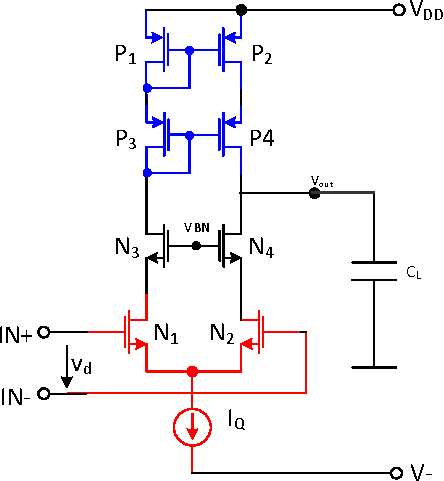
\includegraphics[width=\columnwidth, align=t]{images/11_OTA_einstufig_kaskode.pdf}
\end{minipage}
\hfill
\begin{minipage}[t]{0.62\columnwidth}
    %CHECK: [Simi] @ Flurin: stimmt das so mit den Vorzeichen bei der Verstärkung a ? g_m negativ, r positiv -> a negativ (invertierend)
    \[
        a = g_{\rm m, N1, N2} \cdot \underbrace{ \left( r_{\rm K\_N} \parallel r_{\rm K\_P} \right) }_{r_{\rm out}} 
    \]
    \[
        r_{\rm K\_N, K\_P} \approx r_{\rm DS} \cdot (2+ g_m \cdot r_{\rm DS})
    \]
    \[
        \text{BW} \approx f_d = \frac{1}{2\pi r_{\rm out} C_{L}} \qquad \text{GBW} = f_d \cdot \abs{a} = \frac{g_{\rm m, N1, N2}}{2 \pi C_{L}}
    \]

    \smallskip

    \begin{itemize}
        \item[-] Eingangs- und Ausgangs-Common-Mode-Bereich nicht unabhängig wählbar
        \item[-] Kleinerer Ausgangsspannungsbereich
        \item[+] Geringer Stromverbrauch
        \item[+] Hohe Verstärkung
    \end{itemize}
\end{minipage}


\subsubsection{Folded Cascode OTA}

\begin{minipage}[t]{0.5\columnwidth}
    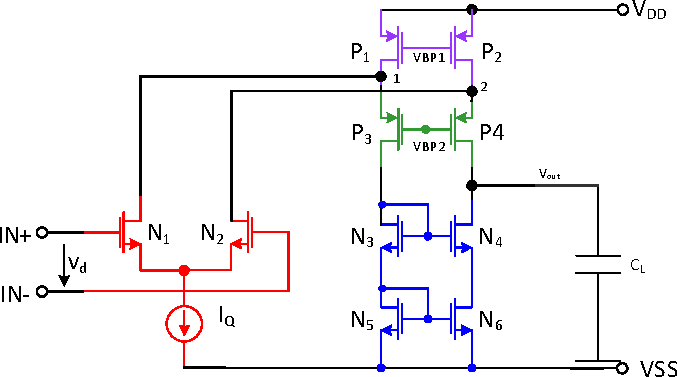
\includegraphics[width=\columnwidth, align=t]{images/11_OTA_einstufig_gefaltete_kaskode.pdf}
\end{minipage}
\hfill
\begin{minipage}[t]{0.48\columnwidth}
    Die Berechnungsformel für die den Folded Cascode OTS sind gleich wie beim Telescopic Cascode OTA. 
    \textrightarrow\ Abschnitt \ref{Telescopic Cascode OTA}

    \smallskip

    \begin{itemize}
        \item[+] Hohe Verstärkung
        \item[+] Eingangs- und Ausgangs-Common- \\
            Mode-Bereich unabhängig wählbar
        \item[-] Hoher Stromverbrauch (meist doppelt im Vergleich zu Telescopic)
    \end{itemize}
\end{minipage}



\subsubsection{Symmetrischer OTA}
\begin{minipage}[t]{0.48\columnwidth}
    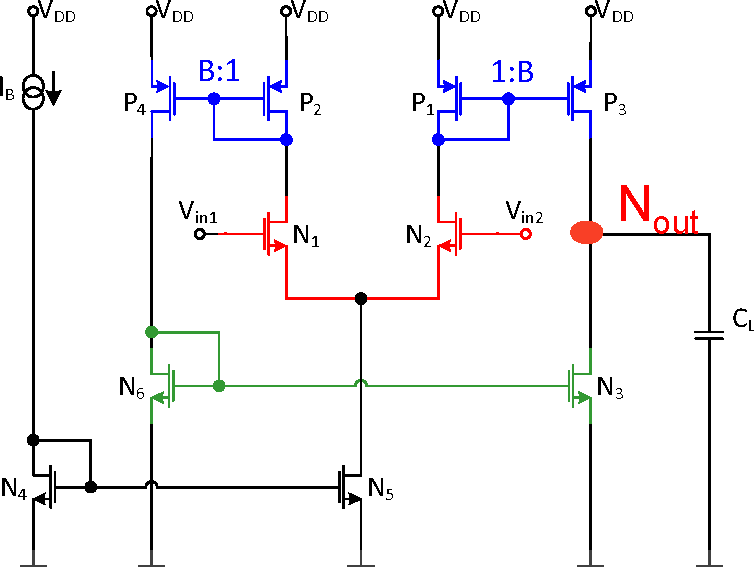
\includegraphics[width=\columnwidth, align=t]{images/11_OTA_einstufig_symmetrisch.pdf}
\end{minipage}
\hfill
\begin{minipage}[t]{0.48\columnwidth}
    %CHECK [Simi] @Flurin: stimmt das so mit den Vorzeichen bei der Verstärkung a? g_m negativ, r positiv -> a negativ (invertierend)
    \[
        a_V = B \cdot  g_{\rm m\_N1} \cdot \left( r_{\rm DS\_N3} \parallel r_{\rm DS\_P3} \right)
    \]
    \[
        f_d = f_{\rm P\_Nout} = \frac{1}{2 \pi \cdot R_{\rm Nout} \cdot C_{\rm Nout}}
    \]
    \[
        f_d \approx \frac{1}{2 \pi \left( r_{\rm DS\_N3} \parallel r_{\rm DS\_P3} \right) C_L}
    \]
    \[
        \text{GBW} = \abs{a_V} \cdot f_d = B \cdot \frac{g_{\rm m\_N1}}{2 \pi C_{\rm Nout}} \approx B \cdot \frac{g_{\rm m\_N1}}{2 \pi C_L}
    \]
\end{minipage}

\smallskip

\begin{itemize}
    \item[+] Besseres Verhalten bei hohen Frequenzkompensation, einstellbar durch $B$
    \item[+] Grosser Aussteuerbereich
    \item[+] Sehr hohe Frequenz des zweiten Pols \textrightarrow\ stabil
\end{itemize}


\subsection{Zweistufige OTA}

\subsubsection{Zweistufiger OTA}

\begin{minipage}[t]{0.5\columnwidth}
    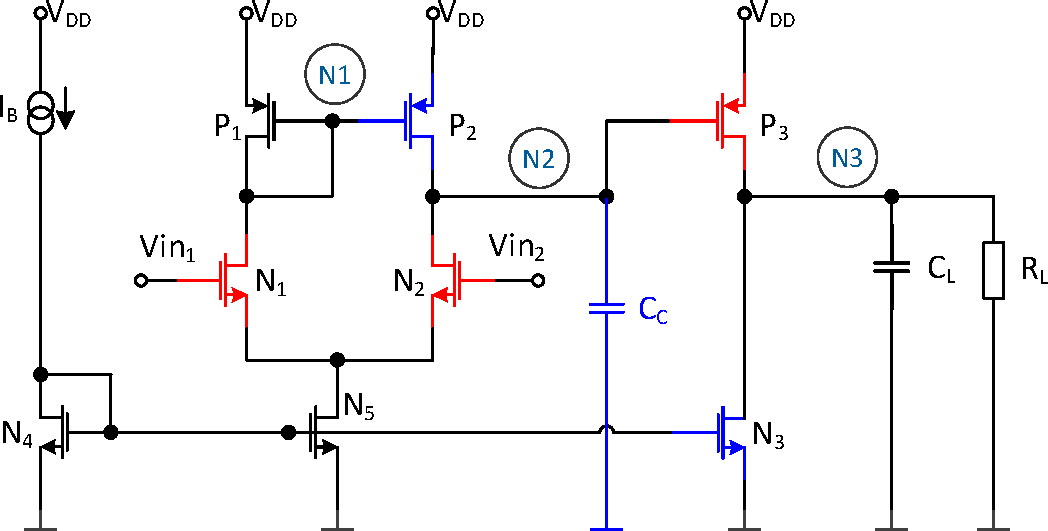
\includegraphics[width=\columnwidth, align=t]{images/11_OTA_zweistufig.pdf}
\end{minipage}
\hfill
\begin{minipage}[t]{0.48\columnwidth}
    \[
        a = \cgn{a_{\rm V1}} \cdot \cvt{a_{\rm V2}} 
    \]
    \[
        \cgn{a_{\rm V1}} = g_{\rm m, N1, N2} (r_{\rm DS\_N2} \parallel r_{\rm DS\_P2})
    \]
    \[
        \cvt{a_{\rm V2}} = g_{\rm m, P3} (\rm r_{DS\_N3} \parallel r_{\rm DS\_P3} \parallel R_L)
    \]
    \[
        f_{\rm p,N2} = \frac{1}{2\pi R_{\rm N2} C_{\rm N2}} \qquad f_{\rm p,N3} = \frac{1}{2\pi R_{L} C_{L}}
    \]
\end{minipage}

\smallskip

\begin{minipage}[t]{0.35\columnwidth}
    \begin{itemize}
        \item[+] Grosse Verstärkung
    \end{itemize}
\end{minipage}
\hfill
\begin{minipage}[t]{0.63\columnwidth}
    \begin{itemize}
        \item[-] $C_2 \gg C_L$ nötig für Stabilität \textrightarrow\ suboptiomal
        \item[-] Durch $C_C$ tiefere Bandbreite
    \end{itemize}
\end{minipage}



\subsubsection{Miller-OTA}

Durch 'Verlagerung' der Kapazität $C_C$ wirkt diese als Miller-Kapazität. 
Somit werden die \textbf{Pole auseinandergeschoben} ohne viel Chipfläche für eine grosse Kapazität zu benötigen.
Die \textbf{Bandbreite} des Miller-OTA ist folglich \textbf{kleiner}, jedoch hat die Eigenschaft der Stabilität das grössere Gewicht.

\smallskip

\begin{minipage}[t]{0.48\columnwidth}
    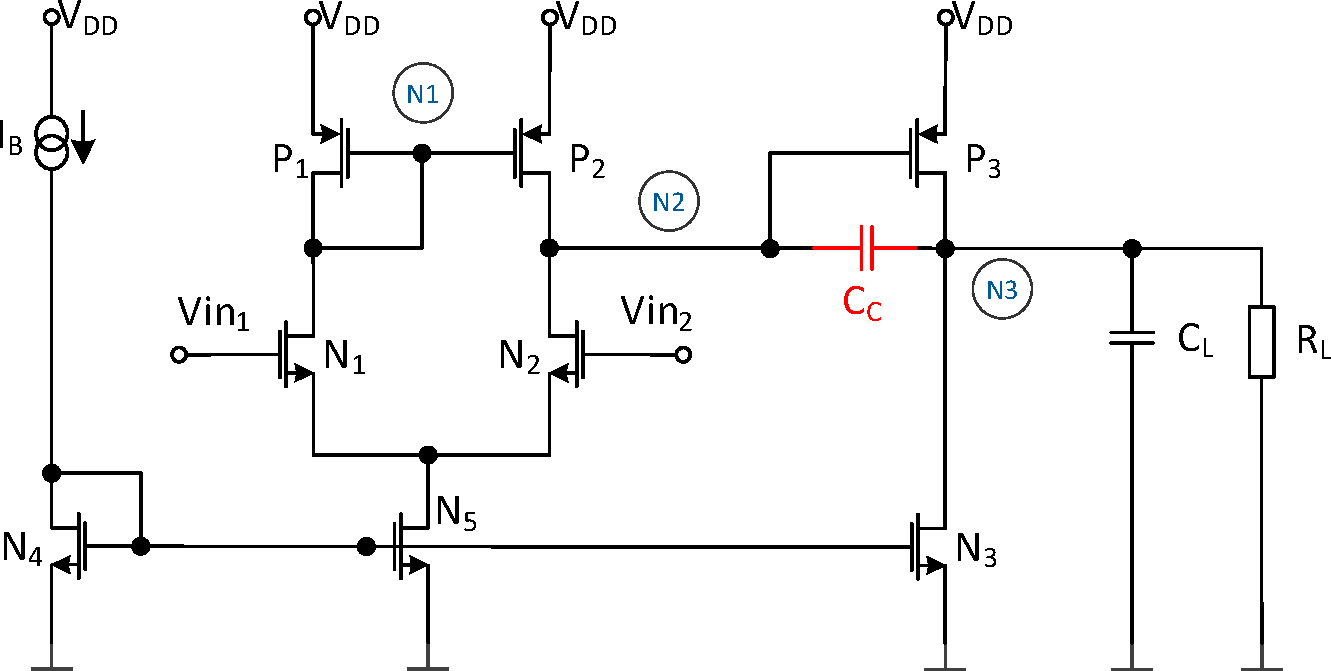
\includegraphics[width=\columnwidth, align=t]{images/11_OTA_zweistufig_miller.pdf}
\end{minipage}
\hfill
\begin{minipage}[t]{0.48\columnwidth}
    \begin{outline}
        \1 \cbl{N2} ist dominierendenr Knoten \textrightarrow\ $f_{\rm pN2}$
        \1 Bei hohe Frequenzen wirkt $C_C$ als Kurzschluss zw. Gate und Drain von $P_3$ \textrightarrow\ Diodenschaltung \textrightarrow\ $f_{\rm pN3}$
        \1 $C_C$ erzeugt eine Nullstelle, deren Lage mit einem $R_C$ in Serie 'platziert' werden kann
    \end{outline} 
\end{minipage}


\renewcommand{\arraystretch}{1.8}
\begin{ctabular}{ll}
    Dominanter Pol                  & $f_{\rm pN2} = \frac{1}{2 \pi R_{\rm N2} \left( C_{\rm N2} + a_{\rm V2} C_C \right)} \approx \frac{1}{2 \pi R_{\rm N2} a_{\rm V2} C_C}$                           \\
    $\qty{3}{\decibel}$-Bandbreite  & $\text{BW} \approx f_d = f_{\rm N2} = \frac{1}{2 \pi R_{\rm N2} a_{\rm V2} C_C}$                                                                                         \\
    Verstärkung $a$                 & $a = \cgn{a_{\rm V1}} \cdot \cvt{a_{\rm V2}} = g_{\rm m\_N1,2} \, R_{\rm N2} \cdot g_{\rm m\_P3} \, R_{\rm N3}$                                                                             \\
    Gain-Bandwidth-Product          & $\text{GBW} = a \cdot f_d = \frac{g_{\rm m\_N1,2} \, R_{\rm N2} \cdot g_{\rm m\_P3} \, R_{\rm N3}}{2 \pi R_{\rm N2} a_{\rm V2} C_C} = \frac{g_{\rm m\_N1,2}}{2 \pi C_C}$ \\ 
    Nicht-Dominanter Pol            & $f_{\rm nd} = f_{\rm N3} = \frac{1}{2 \pi R_{\rm n3} C_L} \approx \frac{g_{\rm m\_P3}}{2 \pi C_L}$                                                                \\ 
    Phasenmarge $\varphi_M$         & $\varphi_M = \qty{90}{\degree} - \arctan \left( \frac{\text{GBW}}{f_{\rm nd}} \right)$                                                                            \\
\end{ctabular}
\renewcommand{\arraystretch}{1}


% \subsubsection{Design-Regeln}
% \begin{itemize}
%     \item $\left. \abs{A(s)F(s)} \right|_{\phi = 180^\circ} < 1$
%     \item $\left. \angle (A(s)F(s)) \right|_{\abs{A(s)F(s)} = 1} > 180^\circ$
%     \item Zweiter Pol bei ca. $3 \cdot GBW$ wählen
% \end{itemize}

